% Options for packages loaded elsewhere
\PassOptionsToPackage{unicode}{hyperref}
\PassOptionsToPackage{hyphens}{url}
%
\documentclass[
]{article}
\usepackage{lmodern}
\usepackage{amssymb,amsmath}
\usepackage{ifxetex,ifluatex}
\ifnum 0\ifxetex 1\fi\ifluatex 1\fi=0 % if pdftex
  \usepackage[T1]{fontenc}
  \usepackage[utf8]{inputenc}
  \usepackage{textcomp} % provide euro and other symbols
\else % if luatex or xetex
  \usepackage{unicode-math}
  \defaultfontfeatures{Scale=MatchLowercase}
  \defaultfontfeatures[\rmfamily]{Ligatures=TeX,Scale=1}
\fi
% Use upquote if available, for straight quotes in verbatim environments
\IfFileExists{upquote.sty}{\usepackage{upquote}}{}
\IfFileExists{microtype.sty}{% use microtype if available
  \usepackage[]{microtype}
  \UseMicrotypeSet[protrusion]{basicmath} % disable protrusion for tt fonts
}{}
\makeatletter
\@ifundefined{KOMAClassName}{% if non-KOMA class
  \IfFileExists{parskip.sty}{%
    \usepackage{parskip}
  }{% else
    \setlength{\parindent}{0pt}
    \setlength{\parskip}{6pt plus 2pt minus 1pt}}
}{% if KOMA class
  \KOMAoptions{parskip=half}}
\makeatother
\usepackage{xcolor}
\IfFileExists{xurl.sty}{\usepackage{xurl}}{} % add URL line breaks if available
\IfFileExists{bookmark.sty}{\usepackage{bookmark}}{\usepackage{hyperref}}
\hypersetup{
  pdftitle={Compulsory exercise 1: Group 12},
  pdfauthor={Emma Skarnes, Håkon Noren and Alexander Johan Arntzen},
  hidelinks,
  pdfcreator={LaTeX via pandoc}}
\urlstyle{same} % disable monospaced font for URLs
\usepackage[margin=1in]{geometry}
\usepackage{color}
\usepackage{fancyvrb}
\newcommand{\VerbBar}{|}
\newcommand{\VERB}{\Verb[commandchars=\\\{\}]}
\DefineVerbatimEnvironment{Highlighting}{Verbatim}{commandchars=\\\{\}}
% Add ',fontsize=\small' for more characters per line
\usepackage{framed}
\definecolor{shadecolor}{RGB}{248,248,248}
\newenvironment{Shaded}{\begin{snugshade}}{\end{snugshade}}
\newcommand{\AlertTok}[1]{\textcolor[rgb]{0.94,0.16,0.16}{#1}}
\newcommand{\AnnotationTok}[1]{\textcolor[rgb]{0.56,0.35,0.01}{\textbf{\textit{#1}}}}
\newcommand{\AttributeTok}[1]{\textcolor[rgb]{0.77,0.63,0.00}{#1}}
\newcommand{\BaseNTok}[1]{\textcolor[rgb]{0.00,0.00,0.81}{#1}}
\newcommand{\BuiltInTok}[1]{#1}
\newcommand{\CharTok}[1]{\textcolor[rgb]{0.31,0.60,0.02}{#1}}
\newcommand{\CommentTok}[1]{\textcolor[rgb]{0.56,0.35,0.01}{\textit{#1}}}
\newcommand{\CommentVarTok}[1]{\textcolor[rgb]{0.56,0.35,0.01}{\textbf{\textit{#1}}}}
\newcommand{\ConstantTok}[1]{\textcolor[rgb]{0.00,0.00,0.00}{#1}}
\newcommand{\ControlFlowTok}[1]{\textcolor[rgb]{0.13,0.29,0.53}{\textbf{#1}}}
\newcommand{\DataTypeTok}[1]{\textcolor[rgb]{0.13,0.29,0.53}{#1}}
\newcommand{\DecValTok}[1]{\textcolor[rgb]{0.00,0.00,0.81}{#1}}
\newcommand{\DocumentationTok}[1]{\textcolor[rgb]{0.56,0.35,0.01}{\textbf{\textit{#1}}}}
\newcommand{\ErrorTok}[1]{\textcolor[rgb]{0.64,0.00,0.00}{\textbf{#1}}}
\newcommand{\ExtensionTok}[1]{#1}
\newcommand{\FloatTok}[1]{\textcolor[rgb]{0.00,0.00,0.81}{#1}}
\newcommand{\FunctionTok}[1]{\textcolor[rgb]{0.00,0.00,0.00}{#1}}
\newcommand{\ImportTok}[1]{#1}
\newcommand{\InformationTok}[1]{\textcolor[rgb]{0.56,0.35,0.01}{\textbf{\textit{#1}}}}
\newcommand{\KeywordTok}[1]{\textcolor[rgb]{0.13,0.29,0.53}{\textbf{#1}}}
\newcommand{\NormalTok}[1]{#1}
\newcommand{\OperatorTok}[1]{\textcolor[rgb]{0.81,0.36,0.00}{\textbf{#1}}}
\newcommand{\OtherTok}[1]{\textcolor[rgb]{0.56,0.35,0.01}{#1}}
\newcommand{\PreprocessorTok}[1]{\textcolor[rgb]{0.56,0.35,0.01}{\textit{#1}}}
\newcommand{\RegionMarkerTok}[1]{#1}
\newcommand{\SpecialCharTok}[1]{\textcolor[rgb]{0.00,0.00,0.00}{#1}}
\newcommand{\SpecialStringTok}[1]{\textcolor[rgb]{0.31,0.60,0.02}{#1}}
\newcommand{\StringTok}[1]{\textcolor[rgb]{0.31,0.60,0.02}{#1}}
\newcommand{\VariableTok}[1]{\textcolor[rgb]{0.00,0.00,0.00}{#1}}
\newcommand{\VerbatimStringTok}[1]{\textcolor[rgb]{0.31,0.60,0.02}{#1}}
\newcommand{\WarningTok}[1]{\textcolor[rgb]{0.56,0.35,0.01}{\textbf{\textit{#1}}}}
\usepackage{longtable,booktabs}
% Correct order of tables after \paragraph or \subparagraph
\usepackage{etoolbox}
\makeatletter
\patchcmd\longtable{\par}{\if@noskipsec\mbox{}\fi\par}{}{}
\makeatother
% Allow footnotes in longtable head/foot
\IfFileExists{footnotehyper.sty}{\usepackage{footnotehyper}}{\usepackage{footnote}}
\makesavenoteenv{longtable}
\usepackage{graphicx,grffile}
\makeatletter
\def\maxwidth{\ifdim\Gin@nat@width>\linewidth\linewidth\else\Gin@nat@width\fi}
\def\maxheight{\ifdim\Gin@nat@height>\textheight\textheight\else\Gin@nat@height\fi}
\makeatother
% Scale images if necessary, so that they will not overflow the page
% margins by default, and it is still possible to overwrite the defaults
% using explicit options in \includegraphics[width, height, ...]{}
\setkeys{Gin}{width=\maxwidth,height=\maxheight,keepaspectratio}
% Set default figure placement to htbp
\makeatletter
\def\fps@figure{htbp}
\makeatother
\setlength{\emergencystretch}{3em} % prevent overfull lines
\providecommand{\tightlist}{%
  \setlength{\itemsep}{0pt}\setlength{\parskip}{0pt}}
\setcounter{secnumdepth}{-\maxdimen} % remove section numbering

\title{Compulsory exercise 1: Group 12}
\usepackage{etoolbox}
\makeatletter
\providecommand{\subtitle}[1]{% add subtitle to \maketitle
  \apptocmd{\@title}{\par {\large #1 \par}}{}{}
}
\makeatother
\subtitle{TMA4268 Statistical Learning V2019}
\author{Emma Skarnes, Håkon Noren and Alexander Johan Arntzen}
\date{20 februar, 2020}

\begin{document}
\maketitle

\hypertarget{problem-1}{%
\section{Problem 1}\label{problem-1}}

For this problem you will need to include some LaTex code. Please
install latex on your computer and then consult Compulsor1.Rmd for hints
how to write formulas in LaTex.

\hypertarget{a}{%
\subsection{a)}\label{a}}

The expected test mean squared error (MSE) at \(x_{0}\) is \[
 E[y_{0} -\hat{f}(x_{0}) ]^{2}.
\]

Where \(y_{0}\) is the new observation.

\hypertarget{b}{%
\subsection{b)}\label{b}}

Firstly, from computation it is clear that

\[
\begin{aligned}
\mathrm{E}[ f( x_{0}) -\hat{f}( x_{0})]^{2} & =\mathrm{E}[ f( x_{0}) -\mathrm{E}[\hat{f}( x_{0})] +\mathrm{E}[\hat{f}( x_{0})] -\hat{f}( x_{0})]^{2} \\
 & =\mathrm{E}[ f( x_{0}) -\mathrm{E}[\hat{f}( x_{0})]]^{2} +2\mathrm{E}[ f( x_{0}) -\mathrm{E}[\hat{f}( x_{0})] \ ][ \mathrm{E}[\hat{f}( x_{0})] -\hat{f}( x_{0})] +\mathrm{E}[ \mathrm{E}[\hat{f}( x_{0})] -\hat{f}( x_{0})]^{2} \\
 & =( f( x_{0}) -\mathrm{E}[\hat{f}( x_{0})])^{2} \  + \mathrm{Var}[ \hat{f}( x_{0})].
\end{aligned}
\]

Secondly note that \(y_0\) and the training data are independent. In
addition \(\mathrm{E[\epsilon]}=0\). Then, expanding the
test\textasciitilde MSE, the decomposition becomes \[
\begin{aligned}
\mathrm{E}[ y_{0} -\hat{f}( x_{0})]^{2} & \ =\mathrm{E}[ f( x_{0}) +\epsilon -\hat{f}( x_{0})]^{2}\\
 & =\mathrm{E}[ \epsilon - \mathrm{E}[ \epsilon ]]^{2} +2\mathrm{E}[ \epsilon ] \mathrm{E}[ f( x_{0}) -\hat{f}( x_{0})] +\mathrm{E}[ f( x_{0}) -\hat{f}( x_{0})]^{2} \ \\
 & =\mathrm{Var}[ \epsilon ] + [ f( x_{0}) - \mathrm{E}[\hat{f}( x_{0})]]^{2}   + \mathrm{Var}[ \hat{f}( x_{0})].
\end{aligned}
\]

\hypertarget{c}{%
\subsection{c)}\label{c}}

Since variance and squared expression cannot be negative each of the
three terms contributes to the expected test MSE at \(x_0\).

The \(\pmb{\mathrm{Var}[ \epsilon ]}\) is the \textbf{irreducible
error}. It is independent of the model and cannot be reduced.

\(\pmb{\mathrm{Var}[ \hat{f}( x_{0})]}\) is the \textbf{variance} of the
prediction at \(x_{0}\). It is a measure of how much the model will
change based on different training data. In general the variance of the
model increases when the the flexibility of the model increases.

\([ f( x_{0}) - \mathrm{E}[\hat{f}( x_{0})]]^{2}\) is the
\textbf{squared bias} at \(x_{0}\), also denoted
\(\mathrm{Bias}(\hat{f}( x_{0}))^{2}\). It is a measure of how much the
model differs from the target function \(f\) at \(x_{0}\). In general a
flexible model will have low bias.

A good model will strike a balance between bias and variance to achieve
a low total expected test MSE.

\hypertarget{d}{%
\subsection{d)}\label{d}}

TRUE, FALSE, FALSE, TRUE

\hypertarget{e}{%
\subsection{e)}\label{e}}

TRUE, FALSE, TRUE, FALSE.

\hypertarget{f}{%
\subsection{f)}\label{f}}

\begin{enumerate}
\def\labelenumi{(\roman{enumi})}
\setcounter{enumi}{1}
\item
\end{enumerate}

\hypertarget{g}{%
\subsection{g)}\label{g}}

C

\hypertarget{problem-2}{%
\section{Problem 2}\label{problem-2}}

\begin{verbatim}
##   Gattung Nummer GEWICHT FANGDATUM MAGENUMF
## 1      Oc     32    0.19  23.09.97     1.56
## 2      Oc     34    0.59  23.09.97     1.63
## 3      Oc     48    0.09  23.09.97     1.69
## 4      Oc     55    0.23  23.09.97     1.69
## 5      Oc     41    0.24  23.09.97     1.75
## 6      Oc     24    0.19  23.09.97     1.81
\end{verbatim}

\hypertarget{a-1}{%
\subsection{a)}\label{a-1}}

The dataset consists of 143 rows and 5 columns, which can be seen from
the \texttt{str()}-function. The qualitative variables are Gattung and
Nummer, while the quantitative variables are GEWICHT, FANGDATUM and
MAGENUMF.

\hypertarget{b-1}{%
\subsection{b)}\label{b-1}}

\begin{Shaded}
\begin{Highlighting}[]
\KeywordTok{ggplot}\NormalTok{(d.worm, }\KeywordTok{aes}\NormalTok{(}\DataTypeTok{x =}\NormalTok{ MAGENUMF, }\DataTypeTok{y =}\NormalTok{ GEWICHT, }\DataTypeTok{colour =}\NormalTok{ Gattung)) }\OperatorTok{+}\StringTok{ }\KeywordTok{geom_point}\NormalTok{() }\OperatorTok{+}\StringTok{ }
\StringTok{    }\KeywordTok{theme_bw}\NormalTok{()}
\end{Highlighting}
\end{Shaded}

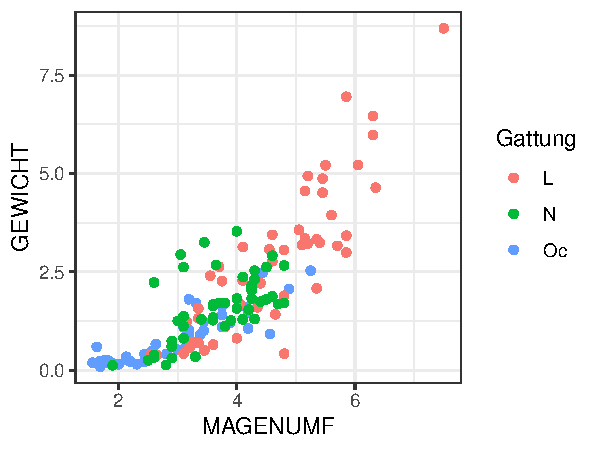
\includegraphics{Project_1_files/figure-latex/unnamed-chunk-3-1.pdf}

The relationship in this scatterplot does not look linear, so we
linearize it by transforming the quantitative variables. Here, we take
the logarithm of both:

\begin{Shaded}
\begin{Highlighting}[]
\KeywordTok{ggplot}\NormalTok{(d.worm, }\KeywordTok{aes}\NormalTok{(}\DataTypeTok{x =} \KeywordTok{log}\NormalTok{(MAGENUMF), }\DataTypeTok{y =} \KeywordTok{log}\NormalTok{(GEWICHT), }\DataTypeTok{colour =}\NormalTok{ Gattung)) }\OperatorTok{+}\StringTok{ }\KeywordTok{geom_point}\NormalTok{() }\OperatorTok{+}\StringTok{ }
\StringTok{    }\KeywordTok{theme_bw}\NormalTok{()}
\end{Highlighting}
\end{Shaded}

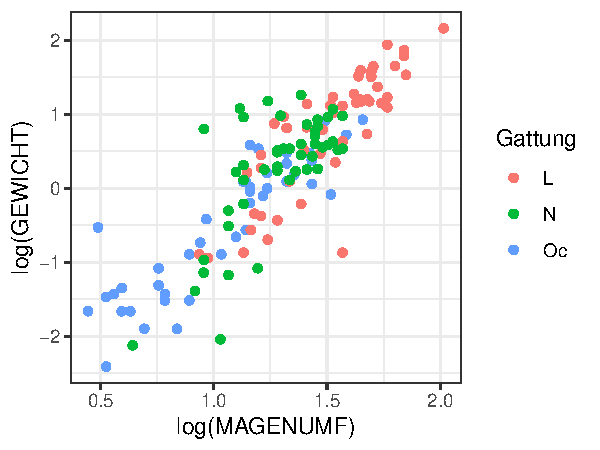
\includegraphics{Project_1_files/figure-latex/unnamed-chunk-4-1.pdf}

The relationship now looks quite linear, which can be seen more clearly
by adding \texttt{+\ geom\textbackslash{}\_smooth(method\ =\ "lm")} to
the \texttt{ggplot()}-function. Especially the species denoted by \(L\)
and \(Oc\) are close to the fitted line, while there is a bigger spread
for the species denoted by \(N\).

\hypertarget{c-1}{%
\subsection{c)}\label{c-1}}

\begin{Shaded}
\begin{Highlighting}[]
\NormalTok{fit.lm =}\StringTok{ }\KeywordTok{lm}\NormalTok{(}\KeywordTok{log}\NormalTok{(GEWICHT) }\OperatorTok{~}\StringTok{ }\KeywordTok{log}\NormalTok{(MAGENUMF) }\OperatorTok{+}\StringTok{ }\NormalTok{Gattung, }\DataTypeTok{data =}\NormalTok{ d.worm)}
\KeywordTok{summary}\NormalTok{(fit.lm)}
\end{Highlighting}
\end{Shaded}

\begin{verbatim}
## 
## Call:
## lm(formula = log(GEWICHT) ~ log(MAGENUMF) + Gattung, data = d.worm)
## 
## Residuals:
##      Min       1Q   Median       3Q      Max 
## -1.79642 -0.25996  0.02864  0.25159  1.40557 
## 
## Coefficients:
##               Estimate Std. Error t value Pr(>|t|)    
## (Intercept)   -3.13865    0.24106 -13.020   <2e-16 ***
## log(MAGENUMF)  2.59310    0.15378  16.862   <2e-16 ***
## GattungN       0.07327    0.10252   0.715    0.476    
## GattungOc     -0.06149    0.12219  -0.503    0.616    
## ---
## Signif. codes:  0 '***' 0.001 '**' 0.01 '*' 0.05 '.' 0.1 ' ' 1
## 
## Residual standard error: 0.4832 on 139 degrees of freedom
## Multiple R-squared:  0.7598, Adjusted R-squared:  0.7547 
## F-statistic: 146.6 on 3 and 139 DF,  p-value: < 2.2e-16
\end{verbatim}

\begin{Shaded}
\begin{Highlighting}[]
\KeywordTok{anova}\NormalTok{(fit.lm)}
\end{Highlighting}
\end{Shaded}

\begin{verbatim}
## Analysis of Variance Table
## 
## Response: log(GEWICHT)
##                Df  Sum Sq Mean Sq  F value Pr(>F)    
## log(MAGENUMF)   1 102.264 102.264 438.0809 <2e-16 ***
## Gattung         2   0.394   0.197   0.8441 0.4321    
## Residuals     139  32.448   0.233                    
## ---
## Signif. codes:  0 '***' 0.001 '**' 0.01 '*' 0.05 '.' 0.1 ' ' 1
\end{verbatim}

The separate equations of the regression models for the three different
species are on the form

\[
\text{log(GEWICHT)} = \hat{\beta_0} + \hat{\beta_1} \cdot \text{log(MAGENUMF)} + \hat{\beta_2} x_{i1} + \hat{\beta_3} x_{i2} + \epsilon_i,
\] where \(x_{i1}\) and \(x_{i2}\) are the dummy variables, given by

\[
  x_{i1} =  
  \begin{cases} 
    1 &\quad \text{if the ith worm is a Nicodrilus} \\
    0 &\quad \text{if the ith worm is not a Nicodrilus}
  \end{cases}
\] \[
  x_{i2} =  
  \begin{cases} 
    1 &\quad \text{if the ith worm is an Octolasion} \\
    0 &\quad \text{if the ith worm is not an Octolasion}
  \end{cases}
\]

This gives the following equations:

\[
  \text{log(GEWICHT)} = 
  \begin{cases} 
    -3.13865 + 2.59310 \cdot \text{log(MAGENUMF)} + 0.24106 &\quad \text{if Gattung="L"} \\
    -3.13865 + 2.59310 \cdot \text{log(MAGENUMF)} + 0.07327 + 0.24106  &\quad \text{if Gattung="N"} \\
    -3.13865 + 2.59310 \cdot \text{log(MAGENUMF)} - 0.06149 + 0.24106  &\quad \text{if Gattung="Oc"}
  \end{cases}
\] By looking at the outputs of the \texttt{summary()} and
\texttt{anova()} functions, we observe that the p-values for the species
are relatively high in the summary, which indicates that there is no
statistical evidence of a difference between the average weight of the
three species - even though it might look like that from our plots. The
anova output has an F-statistic of 0.8441 and associated p-value of
0.4321, which indicates that Gattung is not a relevant predictor.

\hypertarget{d-1}{%
\subsection{d)}\label{d-1}}

\begin{Shaded}
\begin{Highlighting}[]
\CommentTok{# Test interaction term}
\NormalTok{fit.lmInter =}\StringTok{ }\KeywordTok{lm}\NormalTok{(}\KeywordTok{log}\NormalTok{(GEWICHT) }\OperatorTok{~}\StringTok{ }\KeywordTok{log}\NormalTok{(MAGENUMF) }\OperatorTok{*}\StringTok{ }\NormalTok{Gattung, }\DataTypeTok{data =}\NormalTok{ d.worm)}
\KeywordTok{summary}\NormalTok{(fit.lmInter)}
\end{Highlighting}
\end{Shaded}

\begin{verbatim}
## 
## Call:
## lm(formula = log(GEWICHT) ~ log(MAGENUMF) * Gattung, data = d.worm)
## 
## Residuals:
##     Min      1Q  Median      3Q     Max 
## -1.8114 -0.2830  0.0185  0.2457  1.4483 
## 
## Coefficients:
##                         Estimate Std. Error t value Pr(>|t|)    
## (Intercept)             -3.49061    0.42376  -8.237 1.25e-13 ***
## log(MAGENUMF)            2.82702    0.27804  10.168  < 2e-16 ***
## GattungN                 0.19491    0.61075   0.319    0.750    
## GattungOc                0.52368    0.48810   1.073    0.285    
## log(MAGENUMF):GattungN  -0.05431    0.43824  -0.124    0.902    
## log(MAGENUMF):GattungOc -0.45640    0.35462  -1.287    0.200    
## ---
## Signif. codes:  0 '***' 0.001 '**' 0.01 '*' 0.05 '.' 0.1 ' ' 1
## 
## Residual standard error: 0.4831 on 137 degrees of freedom
## Multiple R-squared:  0.7633, Adjusted R-squared:  0.7547 
## F-statistic: 88.36 on 5 and 137 DF,  p-value: < 2.2e-16
\end{verbatim}

\begin{Shaded}
\begin{Highlighting}[]
\KeywordTok{anova}\NormalTok{(fit.lmInter, fit.lm)}
\end{Highlighting}
\end{Shaded}

\begin{verbatim}
## Analysis of Variance Table
## 
## Model 1: log(GEWICHT) ~ log(MAGENUMF) * Gattung
## Model 2: log(GEWICHT) ~ log(MAGENUMF) + Gattung
##   Res.Df    RSS Df Sum of Sq      F Pr(>F)
## 1    137 31.978                           
## 2    139 32.448 -2  -0.46928 1.0052 0.3686
\end{verbatim}

Here, the p-value are also relatively far away from zero, and the
F-statistic from the anova table is close to 1, both of which supports
our results from \(\textbf{2c)}\). In other words, an interaction term
between the logarithm of the circumference and the species does not
improve the model.

\hypertarget{e-1}{%
\subsection{e)}\label{e-1}}

\begin{Shaded}
\begin{Highlighting}[]
\KeywordTok{autoplot}\NormalTok{(fit.lm)  }\CommentTok{# Residual analysis on our regression model}
\end{Highlighting}
\end{Shaded}

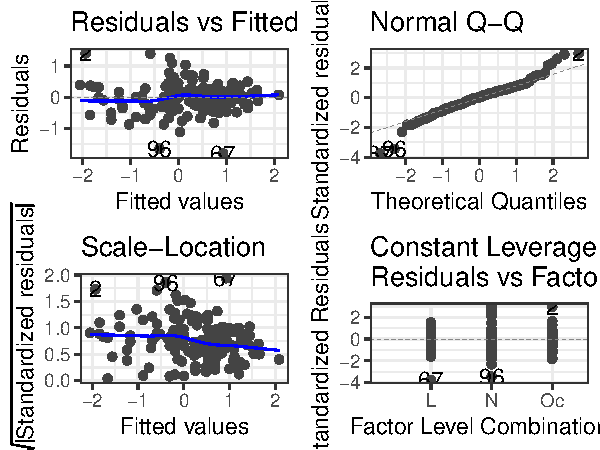
\includegraphics{Project_1_files/figure-latex/unnamed-chunk-7-1.pdf}

The Residuals vs.~fitted plot, or Tukey-Anscombe, seems to be nonlinear,
which is how we want the residuals to behave. We have some outliers in
the QQ-plot, especially points 7, 96 and 2. However, the majority of the
points are making up a fairly straight line, so some outliers does not
imply that our assumptions are violated. In the Scale-Location plot, the
points seems to gather a little bit as the fitted values increase. This
can be a sign of non-equal variances, which is violating our
assumptions. In the Constant Leverage: Residuals vs Factor Levels plot,
we can see that the spread of the points seems to differ based on the
species. While there is only one obvious outlier for the Lumbricus
species, there are more outliers for the two other species, even though
these are not as far from the majority as the outlier in L. Also, note
that the same observations from the QQ-plot seems to be the problematic
ones.

\begin{Shaded}
\begin{Highlighting}[]
\CommentTok{# Compare to the model without transformed variables}
\NormalTok{fit.lm1 =}\StringTok{ }\KeywordTok{lm}\NormalTok{(GEWICHT }\OperatorTok{~}\StringTok{ }\NormalTok{MAGENUMF }\OperatorTok{+}\StringTok{ }\NormalTok{Gattung, }\DataTypeTok{data =}\NormalTok{ d.worm)}
\KeywordTok{autoplot}\NormalTok{(fit.lm1, }\DataTypeTok{smooth.colour =} \OtherTok{NA}\NormalTok{)}
\end{Highlighting}
\end{Shaded}

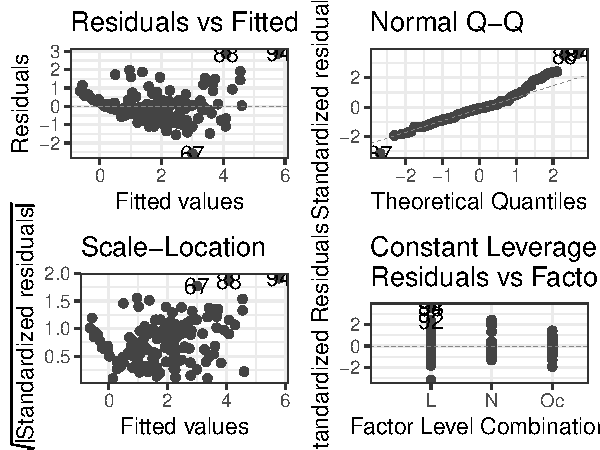
\includegraphics{Project_1_files/figure-latex/unnamed-chunk-8-1.pdf}

Comparing our model with transformed variables to the model without any
transformations, we can clearly see that the latter one is violating the
assumptions more. There seems to be a trend in the Tukey-Anscombe plot,
and the points are not following the line quite as well in the QQ-plot.
However, the Scale-Location plot does not behave as in our transformed
model - here the points are fairly well distributed. We do have some
outliers and problematic observations in the Leverage plot, but they are
in general more gathered here than in the model we have used.

\hypertarget{f-1}{%
\subsection{f)}\label{f-1}}

It is important to carry out a residual analysis since we should verify
that the underlying assumptions are not violated - if they are so, the
model is not valid. In case of violated assumptions, we can for instance
remove the outliers and fit the model over again, or we can try other
transformations of the predictor value(s).

\hypertarget{g-1}{%
\subsection{g)}\label{g-1}}

FALSE, FALSE, FALSE, TRUE.

\hypertarget{problem-3}{%
\section{Problem 3}\label{problem-3}}

In this problem, we will use a dataset from the Wimbledon tennis
tournament andpredict the result for player 1 (win=1 or loose=0) based
on data from the match.

\hypertarget{a-2}{%
\subsection{a)}\label{a-2}}

Probability to win for player 1 given by a logistic regression model:

\[
P(Y_i = 1| {\bf X}={\boldsymbol{x}}_i) = p_i = \frac{e^{\beta_0 + \beta_1x_{i1} + \beta_2 x_{i2} + \beta_3x_{i3} + \beta_4 x_{i4}}}{ 1+ e^{\beta_0 + \beta_1x_{i1} + \beta_2x_{i2}+ \beta_3x_{i3} + \beta_4 x_{i4}}}
\]

We first define

\[
\beta_0 + \beta_1x_{i1} + \beta_2 x_{i2} + \beta_3x_{i3} + \beta_4 x_{i4} = \beta x
\]

Furthermore we know that

\[
\begin{aligned}
1-p_i &= 1 - \frac{e^{\beta x}}{1+e^{\beta x}} \\
&= \frac{1 + e^{\beta x} - e^{\beta x}}{1+e^{\beta x}} \\
&= \frac{1}{1+e^{\beta x}}
\end{aligned}
\]

Hence we find the linear relation between \(p_i\) and the covariates:

\[
\begin{aligned}
\text{logit}(p_i) &= \log(\dfrac{p_i}{1-p_i}) \\
&=  \log(p_i) - \log({1 - p_i}) \\
&=  \log(e^{\beta x}) - \log(1 + e^{\beta x}) - \log(1) + \log({1 + e^{\beta x}}) \\
&= \beta x - 0 \\
&= \beta_0 + \beta_1x_{i1} + \beta_2 x_{i2} + \beta_3x_{i3} + \beta_4 x_{i4}
\end{aligned}
\]

\hypertarget{b-2}{%
\subsection{b)}\label{b-2}}

We provide an interpretation of how the coefficients \(\beta_i\) affect
\(p_i\) by looking at the relative change in odds \(\frac{p_i}{1-p_i}\)
when increasing a covariate \(\beta_i\).

\[
\begin{aligned}
\frac{\text{odds}(Y_i=1 \mid X_{1} = x_{i1} + 1)}{\text{odds}(Y_i=1 \mid X_j = x_{ij})} &= \frac{e^{\beta_0 + \beta_1 (x_{i1} + 1) + \beta_2 x_{i2} + \beta_3x_{i3} + \beta_4 x_{i4}}}{e^{\beta_0 + \beta_1x_{i1} + \beta_2 x_{i2} + \beta_3x_{i3} + \beta_4 x_{i4}}} \\
&= e^{\beta_11}
\end{aligned}
\]

Hence we see that the odds will increase with a factor of
\(e^{\beta_1}\) if player 1 has one more ace, \(x_{i1}' = x_{i1} + 1\).
As \(\beta_1 = 0.36338\) we know that one more ace for player 1 will
increase the likelihood for player 1 winning the match with a factor of
\(e^{0.36338} \approx 1.438\), in our model.

\begin{verbatim}
##                Estimate Std. Error     z value     Pr(>|z|)
## (Intercept) -0.02437712 0.59301536 -0.04110706 0.9672105452
## ACE.1        0.36338363 0.10136157  3.58502352 0.0003370478
## ACE.2       -0.22388414 0.07369365 -3.03803855 0.0023812349
## UFE.1       -0.09846814 0.02840389 -3.46671307 0.0005268640
## UFE.2        0.09010020 0.02478616  3.63510142 0.0002778713
\end{verbatim}

\hypertarget{c-2}{%
\subsection{c)}\label{c-2}}

We will now use a \(0.5\) cutoff rule, meaning we classify an
observation \(\boldsymbol{x}\) as a win for player 1 if
\(P(Y = 1 | x) > 0.5\). We find the boundary from

\[
\begin{aligned}
P(Y_i = 1| {\bf X}={\boldsymbol{x}}_i) &= p_i \\
&= \frac{e^{\beta x}}{ 1+ e^{\beta x}} = 0.5 \\
&\implies e^{\beta x} = 1 \\   
&\implies \beta_0 + \beta_1 x_{1} + \beta_2 x_{2} = 0 \\
&\implies x_2 = -\frac{\beta_1}{\beta_2}x_1 - \frac{\beta_0}{\beta_2}
\end{aligned}
\] Hence we can plot the line \(y = ax + b\) with
\(a = -\frac{\beta_1}{\beta_2}\) and \(b = -\frac{\beta_0}{\beta_2}\).

We can now provide a plot with \texttt{ACEdiff} as x-axis,
\texttt{UFEdiff} as y-axis, color the points to indicate win or loss
together with our computed boundary. This gives a visual understanding
of our classification model.

\begin{Shaded}
\begin{Highlighting}[]
\CommentTok{# make variables for difference}
\NormalTok{tennis}\OperatorTok{$}\NormalTok{ACEdiff =}\StringTok{ }\NormalTok{tennis}\OperatorTok{$}\NormalTok{ACE}\FloatTok{.1} \OperatorTok{-}\StringTok{ }\NormalTok{tennis}\OperatorTok{$}\NormalTok{ACE}\FloatTok{.2}
\NormalTok{tennis}\OperatorTok{$}\NormalTok{UFEdiff =}\StringTok{ }\NormalTok{tennis}\OperatorTok{$}\NormalTok{UFE}\FloatTok{.1} \OperatorTok{-}\StringTok{ }\NormalTok{tennis}\OperatorTok{$}\NormalTok{UFE}\FloatTok{.2}

\CommentTok{# divide into test and train set}
\NormalTok{n =}\StringTok{ }\KeywordTok{dim}\NormalTok{(tennis)[}\DecValTok{1}\NormalTok{]}
\NormalTok{n2 =}\StringTok{ }\NormalTok{n}\OperatorTok{/}\DecValTok{2}
\KeywordTok{set.seed}\NormalTok{(}\DecValTok{1111}\NormalTok{)  }\CommentTok{# to reproduce the same test and train sets each time you run the code}
\NormalTok{train =}\StringTok{ }\KeywordTok{sample}\NormalTok{(}\KeywordTok{c}\NormalTok{(}\DecValTok{1}\OperatorTok{:}\NormalTok{n), }\DataTypeTok{replace =}\NormalTok{ F)[}\DecValTok{1}\OperatorTok{:}\NormalTok{n2]}
\NormalTok{tennisTest =}\StringTok{ }\NormalTok{tennis[}\OperatorTok{-}\NormalTok{train, ]}
\NormalTok{tennisTrain =}\StringTok{ }\NormalTok{tennis[train, ]}
\end{Highlighting}
\end{Shaded}

\begin{Shaded}
\begin{Highlighting}[]
\NormalTok{r.tennisLogres =}\StringTok{ }\KeywordTok{glm}\NormalTok{(Result }\OperatorTok{~}\StringTok{ }\NormalTok{ACEdiff }\OperatorTok{+}\StringTok{ }\NormalTok{UFEdiff, }\DataTypeTok{data =}\NormalTok{ tennisTrain, }\DataTypeTok{family =} \StringTok{"binomial"}\NormalTok{)}

\NormalTok{beta =}\StringTok{ }\NormalTok{r.tennisLogres}\OperatorTok{$}\NormalTok{coefficients}
\NormalTok{a =}\StringTok{ }\OperatorTok{-}\NormalTok{beta[}\DecValTok{1}\NormalTok{]}\OperatorTok{/}\NormalTok{beta[}\DecValTok{3}\NormalTok{]}
\NormalTok{b =}\StringTok{ }\OperatorTok{-}\NormalTok{beta[}\DecValTok{2}\NormalTok{]}\OperatorTok{/}\NormalTok{beta[}\DecValTok{3}\NormalTok{]}

\NormalTok{plot =}\StringTok{ }\KeywordTok{ggplot}\NormalTok{(tennisTrain, }\KeywordTok{aes}\NormalTok{(}\DataTypeTok{x =}\NormalTok{ ACEdiff, }\DataTypeTok{y =}\NormalTok{ UFEdiff, }\DataTypeTok{color =}\NormalTok{ Result)) }\OperatorTok{+}\StringTok{ }\KeywordTok{geom_point}\NormalTok{() }\OperatorTok{+}\StringTok{ }
\StringTok{    }\KeywordTok{geom_abline}\NormalTok{(}\DataTypeTok{slope =}\NormalTok{ b, }\DataTypeTok{intercept =}\NormalTok{ a) }\OperatorTok{+}\StringTok{ }\KeywordTok{theme_bw}\NormalTok{()}

\NormalTok{plot}
\end{Highlighting}
\end{Shaded}

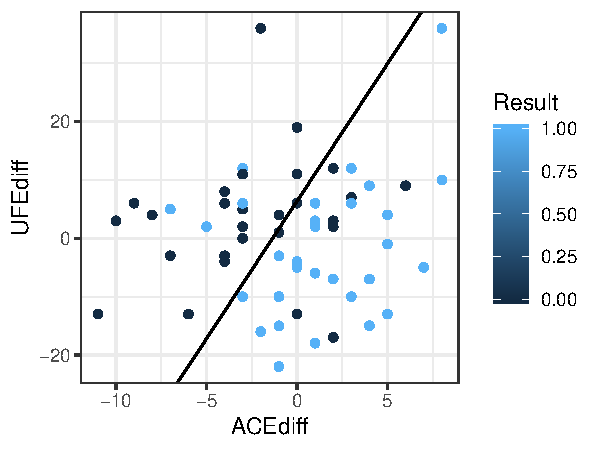
\includegraphics{Project_1_files/figure-latex/unnamed-chunk-12-1.pdf}

Furthermore we can use our model to predict win or loss by player 1 on
the test set. As our data set includes the row \texttt{Result} we know
whether player 1 actually won or not. Hence we find the confusion matrix
to measure the accuracy of our model. This also enables us to find the
sensitivity and specificity. If \(TP\) are true positives, \(P\) the sum
of predicted and actual positives, \(TN\) are true negatives, \(N\) the
sum of predicted and actual negatives, we have sensitivity given by:

\[
\frac{\text{TP}}{\text{P}}
\]

And specificity by:

\[
\frac{\text{TN}}{\text{N}}
\]

\begin{verbatim}
##     pred
## real  0  1
##    0 16 12
##    1  5 26
\end{verbatim}

\begin{verbatim}
## [1] "Sensitivity: 0.838709677419355"
\end{verbatim}

\begin{verbatim}
## [1] "Specificity: 0.571428571428571"
\end{verbatim}

\hypertarget{d-2}{%
\subsection{d)}\label{d-2}}

We will now use Linear discriminant analysis (LDA) to classify in the
same manner as we did above. Using LDA we assume that our data follow
known normal distributions, and we use Bayes theorem to find \(P(Y|X)\).
Given that we have \(K\) classes we find the posterior probability by

\[
P(Y=k | {\bf X}={\boldsymbol x}) = \frac{\pi_k f_k({\boldsymbol x})}{\sum_{l=1}^K \pi_l f_l({\boldsymbol x})}
\]

First of all we have \(\pi_k = P(Y = k)\) which is called the
\emph{prior probability}. In our case \(\pi_1\) is the probability for
player 1 winning any match, and \(\pi_0\) is the probability for loss.
Given a data set, as we have from \texttt{tennis}, we estimate
\(\hat\pi_1\) by dividing total number of wins \(n_w\) by total number
of losses \(n_l\) by player 1:

\[
\hat{\pi_1} = \dfrac{n_w}{n_l}
\]

\(\mu_k\) is the expectation of the covariate \(x\) for the different
classes. In our case \(x\) is a multivariate random vector with two
random variables \(x = [x_1,x_2]^T\). \(x_1\) represents
\texttt{ACEdiff} and \(x_2\) \texttt{UFEdiff}. \(\mu_1\) is the
expecation of \(x\) given \(Y = 1\), meaning player 1 won the match,
\(\text{E}[x|Y = 1]\), in the same way \(\mu_0\) is the expecation of
\(x\) in the cases where player 1 lost the match, \(\text{E}[x|Y = 0]\).
\(\mu_k\) is estimated by

\[
\hat{\boldsymbol{\mu}}_1 = \frac{1}{n_w}\sum_{i:y_i=1} {\bf X}_i
\]

\(\Sigma\) is the covariance matrix for \(x\), or for \texttt{ACEdiff}
and \texttt{UFEdiff}, our random variables in this case. With a given
data set we have the covariance matrix for class \(k\):

\[
\hat{\boldsymbol{\Sigma}}_k=\frac{1}{n_k-1}\sum_{i:y_i=k} ({\bf X}_i-\hat{\boldsymbol{\mu}}_k ) ({\bf X}_i-\hat{\boldsymbol{\mu}}_k)^T
\]

Which we use to find the use the following estimator for the covariance

\[
\hat{\boldsymbol{\Sigma}}= \sum_{k=1}^K \frac{n_k - 1}{n - K} \cdot \hat{\boldsymbol{\Sigma}}_k
\]

Finally we have the class conditional distributions
\(f_k(\boldsymbol x) =\text{P}(\boldsymbol X =\boldsymbol x|Y = k)\).
These are in the case of LDA and QDA assumed to be normal. This is the
distribution of all \(x\) that belongs to class \(k\). Again, for the
tennis problem \(f_0(\boldsymbol x)\) gives the distribution for the
bivariate variable \(\boldsymbol x = [\text{ACEdiff,UFEdiff}]^T\) in the
case where player 1 lost, and \(f_1(\boldsymbol x)\) in the case where
player 1 won.

\hypertarget{e-2}{%
\subsection{e)}\label{e-2}}

\textbf{Expression }

We will now derive an expression for
\(\delta_0({\boldsymbol x}) = \delta_1({\boldsymbol x})\) starting with

\[
\begin{aligned}
P(Y=0 | {\bf X}={\boldsymbol x}) &= P(Y=1 | {\bf X}={\boldsymbol x}) \\
\\
\frac{\pi_0 f_0({\boldsymbol x})}{\pi_0 f_0({\boldsymbol x}) + \pi_1 f_1({\boldsymbol x})} 
&= \frac{\pi_1 f_1({\boldsymbol x})}{\pi_0 f_0({\boldsymbol x}) + \pi_1 f_1({\boldsymbol x})} \\
\\
\pi_0 f_0({\boldsymbol x})
&= \pi_1 f_1({\boldsymbol x})
\end{aligned}
\]

Where \(f_k(\boldsymbol{x})\) is defined as

\[
f_k({\boldsymbol x}) = \frac{1}{(2 \pi)^{p/2}|\boldsymbol{\Sigma}|^{1/2}}e^{-\dfrac{1}{2}({\boldsymbol x}-\boldsymbol{\mu_k})^T \boldsymbol{\Sigma}^{-1}({\boldsymbol x}-\boldsymbol{\mu_k})}
\]

We see that the term outside the exponent cancels because of the
assumption that \(\Sigma_0 = \Sigma_1 = \Sigma\), hence we take \(\log\)
on both sides to get:

\[
\begin{aligned}
-\dfrac{1}{2}({\boldsymbol x}-\boldsymbol{\mu_0})^T \boldsymbol{\Sigma}^{-1}({\boldsymbol x}-\boldsymbol{\mu_0}) + \log\pi_0
&= -\dfrac{1}{2}({\boldsymbol x}-\boldsymbol{\mu_1})^T \boldsymbol{\Sigma}^{-1}({\boldsymbol x}-\boldsymbol{\mu_1}) + \log\pi_1 \\
\end{aligned}
\]

Finally terms independent of \(k\) cancels, like \(x^T\Sigma^{-1}x\).
Furthermore, by the symmetry of \(\Sigma\) and the fact that \(b^T = b\)
when \(b \in \mathbb{R}\) we get

\[
\begin{aligned}
{\boldsymbol x}^T \boldsymbol{\Sigma}^{-1}\boldsymbol{\mu}_0 - \frac{1}{2}\boldsymbol{\mu}_0^T \boldsymbol{\Sigma}^{-1}\boldsymbol{\mu}_0 + \log \pi_0
&=
{\boldsymbol x}^T \boldsymbol{\Sigma}^{-1}\boldsymbol{\mu}_1 - \frac{1}{2}\boldsymbol{\mu}_1^T \boldsymbol{\Sigma}^{-1}\boldsymbol{\mu}_1 + \log \pi_1 \\
\delta_0({\boldsymbol x}) &= \delta_1({\boldsymbol x})
\end{aligned}
\]

\textbf{Function for class boundary}

We will now derive the class boundary by using the expression we have
derived above. As we know that \[
P(Y=0 | {\bf X}={\boldsymbol x}) = P(Y=1 | {\bf X}={\boldsymbol x}) = 0.5
\]

We can use \(\delta_0({\boldsymbol x}) = \delta_1({\boldsymbol x})\) to
find

\[
{\boldsymbol x}^T\boldsymbol{\Sigma}^{-1}(\boldsymbol\mu_0 -\boldsymbol\mu_1)-\frac{1}{2}\boldsymbol\mu_0^T \boldsymbol{\Sigma}^{-1}\boldsymbol\mu_0 +\frac{1}{2}\boldsymbol\mu_1^T \boldsymbol{\Sigma}^{-1}\boldsymbol\mu_1 +\log\dfrac{ \pi_0}{ \pi_1}=0
\]

By defining

\[
[\alpha_1,\alpha_2] = \boldsymbol{\Sigma}^{-1}(\boldsymbol\mu_0 -\boldsymbol\mu_1)
\]

we get

\[
[x_1,x_2]^T[\alpha_1,\alpha_2] = x_1\alpha_1 + x_2\alpha_2
\]

and finally we have

\[
x_2 
= x_1\frac{\alpha_1}{\alpha_2} + \frac{1}{2\alpha_2}
(\boldsymbol\mu_0^T \boldsymbol{\Sigma}^{-1}\boldsymbol\mu_0 
-\boldsymbol\mu_1^T \boldsymbol{\Sigma}^{-1}\boldsymbol\mu_1 -2\log\dfrac{ \pi_0}{ \pi_1})
\]

\begin{Shaded}
\begin{Highlighting}[]
\NormalTok{n =}\StringTok{ }\KeywordTok{nrow}\NormalTok{(tennisTrain)}

\NormalTok{r1 =}\StringTok{ }\NormalTok{tennisTrain[tennisTrain}\OperatorTok{$}\NormalTok{Result }\OperatorTok{==}\StringTok{ }\DecValTok{1}\NormalTok{, ]}
\NormalTok{r1 =}\StringTok{ }\KeywordTok{select}\NormalTok{(r1, ACEdiff, UFEdiff)}
\NormalTok{mu1 =}\StringTok{ }\KeywordTok{colMeans}\NormalTok{(r1)}
\NormalTok{cov1 =}\StringTok{ }\KeywordTok{cov}\NormalTok{(r1)}
\NormalTok{pi1 =}\StringTok{ }\KeywordTok{nrow}\NormalTok{(r1)}\OperatorTok{/}\NormalTok{n}

\NormalTok{r0 =}\StringTok{ }\NormalTok{tennisTrain[tennisTrain}\OperatorTok{$}\NormalTok{Result }\OperatorTok{==}\StringTok{ }\DecValTok{0}\NormalTok{, ]}
\NormalTok{r0 =}\StringTok{ }\KeywordTok{select}\NormalTok{(r0, ACEdiff, UFEdiff)}
\NormalTok{mu0 =}\StringTok{ }\KeywordTok{colMeans}\NormalTok{(r0)}
\NormalTok{cov0 =}\StringTok{ }\KeywordTok{cov}\NormalTok{(r0)}
\NormalTok{pi0 =}\StringTok{ }\KeywordTok{nrow}\NormalTok{(r0)}\OperatorTok{/}\NormalTok{n}

\NormalTok{covEst =}\StringTok{ }\NormalTok{(}\DecValTok{1}\OperatorTok{/}\NormalTok{(n }\OperatorTok{-}\StringTok{ }\DecValTok{2}\NormalTok{)) }\OperatorTok{*}\StringTok{ }\NormalTok{((}\KeywordTok{nrow}\NormalTok{(r0) }\OperatorTok{-}\StringTok{ }\DecValTok{1}\NormalTok{) }\OperatorTok{*}\StringTok{ }\NormalTok{cov0 }\OperatorTok{+}\StringTok{ }\NormalTok{((}\KeywordTok{nrow}\NormalTok{(r1) }\OperatorTok{-}\StringTok{ }\DecValTok{1}\NormalTok{) }\OperatorTok{*}\StringTok{ }\NormalTok{cov1))}
\NormalTok{covInv =}\StringTok{ }\KeywordTok{solve}\NormalTok{(covEst)}

\NormalTok{alpha =}\StringTok{ }\NormalTok{covInv }\OperatorTok\StringTok{ }\NormalTok{(mu0 }\OperatorTok{-}\StringTok{ }\NormalTok{mu1)}
\NormalTok{a =}\StringTok{ }\OperatorTok{-}\NormalTok{alpha[}\DecValTok{1}\NormalTok{]}\OperatorTok{/}\NormalTok{alpha[}\DecValTok{2}\NormalTok{]}
\NormalTok{b =}\StringTok{ }\NormalTok{(}\DecValTok{1}\OperatorTok{/}\NormalTok{(}\DecValTok{2} \OperatorTok{*}\StringTok{ }\NormalTok{alpha[}\DecValTok{2}\NormalTok{])) }\OperatorTok{*}\StringTok{ }\NormalTok{(}\KeywordTok{t}\NormalTok{(mu0) }\OperatorTok\StringTok{ }\NormalTok{covInv }\OperatorTok\StringTok{ }\NormalTok{mu0 }\OperatorTok{-}\StringTok{ }\KeywordTok{t}\NormalTok{(mu1) }\OperatorTok\StringTok{ }\NormalTok{covInv }\OperatorTok\StringTok{ }\NormalTok{mu1 }\OperatorTok{-}\StringTok{ }
\StringTok{    }\DecValTok{2} \OperatorTok{*}\StringTok{ }\KeywordTok{log}\NormalTok{(pi0}\OperatorTok{/}\NormalTok{pi1))}

\NormalTok{plot =}\StringTok{ }\KeywordTok{ggplot}\NormalTok{(tennisTest, }\KeywordTok{aes}\NormalTok{(}\DataTypeTok{x =}\NormalTok{ ACEdiff, }\DataTypeTok{y =}\NormalTok{ UFEdiff, }\DataTypeTok{color =}\NormalTok{ Result)) }\OperatorTok{+}\StringTok{ }\KeywordTok{geom_point}\NormalTok{() }\OperatorTok{+}\StringTok{ }
\StringTok{    }\KeywordTok{geom_abline}\NormalTok{(}\DataTypeTok{slope =}\NormalTok{ a, }\DataTypeTok{intercept =}\NormalTok{ b) }\OperatorTok{+}\StringTok{ }\KeywordTok{theme_bw}\NormalTok{()}

\NormalTok{plot}
\end{Highlighting}
\end{Shaded}

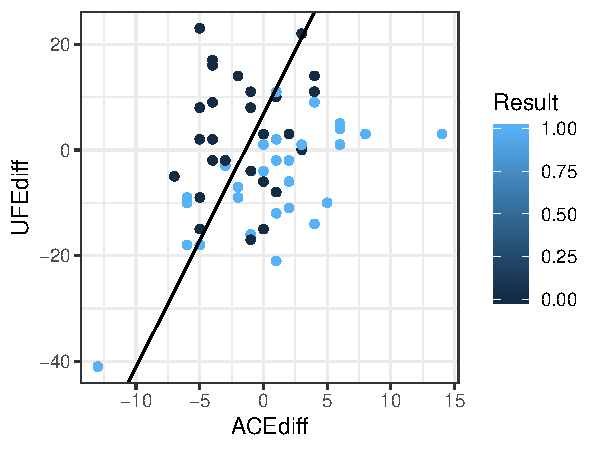
\includegraphics{Project_1_files/figure-latex/unnamed-chunk-14-1.pdf}

\hypertarget{f-2}{%
\subsection{f)}\label{f-2}}

\begin{Shaded}
\begin{Highlighting}[]
\NormalTok{r.tennisLDA =}\StringTok{ }\KeywordTok{lda}\NormalTok{(Result }\OperatorTok{~}\StringTok{ }\NormalTok{ACEdiff }\OperatorTok{+}\StringTok{ }\NormalTok{UFEdiff, }\DataTypeTok{data =}\NormalTok{ tennisTrain)}
\NormalTok{tennisLDAPred =}\StringTok{ }\KeywordTok{predict}\NormalTok{(r.tennisLDA, tennisTest)}\OperatorTok{$}\NormalTok{class}

\NormalTok{tennisLDACM =}\StringTok{ }\KeywordTok{table}\NormalTok{(}\DataTypeTok{real =}\NormalTok{ tennisTest}\OperatorTok{$}\NormalTok{Result, }\DataTypeTok{predicted =}\NormalTok{ tennisLDAPred)}
\NormalTok{tennisLDACM}
\end{Highlighting}
\end{Shaded}

\begin{verbatim}
##     predicted
## real  0  1
##    0 16 12
##    1  5 26
\end{verbatim}

\begin{Shaded}
\begin{Highlighting}[]
\NormalTok{sensLDA =}\StringTok{ }\NormalTok{tennisLDACM[}\DecValTok{2}\NormalTok{, }\DecValTok{2}\NormalTok{]}\OperatorTok{/}\KeywordTok{sum}\NormalTok{(tennisLDACM[}\DecValTok{2}\NormalTok{, ])}
\KeywordTok{print}\NormalTok{(}\KeywordTok{paste0}\NormalTok{(}\StringTok{"Sensitivity: "}\NormalTok{, sensLDA))}
\end{Highlighting}
\end{Shaded}

\begin{verbatim}
## [1] "Sensitivity: 0.838709677419355"
\end{verbatim}

\begin{Shaded}
\begin{Highlighting}[]
\NormalTok{specLDA =}\StringTok{ }\NormalTok{tennisLDACM[}\DecValTok{1}\NormalTok{, }\DecValTok{1}\NormalTok{]}\OperatorTok{/}\KeywordTok{sum}\NormalTok{(tennisLDACM[}\DecValTok{1}\NormalTok{, ])}
\KeywordTok{print}\NormalTok{(}\KeywordTok{paste0}\NormalTok{(}\StringTok{"Specificity: "}\NormalTok{, specLDA))}
\end{Highlighting}
\end{Shaded}

\begin{verbatim}
## [1] "Specificity: 0.571428571428571"
\end{verbatim}

\hypertarget{g-2}{%
\subsection{g)}\label{g-2}}

When we derived the decision boundary for LDA we assumed that each class
have equal covariance matrices. For QDA we do not assume this and hence
the quadratic terms of \(x\) do not cancel and we obviously get a
decision boundary that is quadratic.

\begin{Shaded}
\begin{Highlighting}[]
\NormalTok{r.tennisQDA =}\StringTok{ }\KeywordTok{qda}\NormalTok{(Result }\OperatorTok{~}\StringTok{ }\NormalTok{ACEdiff }\OperatorTok{+}\StringTok{ }\NormalTok{UFEdiff, }\DataTypeTok{data =}\NormalTok{ tennisTrain)}
\NormalTok{tennisQDAPred =}\StringTok{ }\KeywordTok{predict}\NormalTok{(r.tennisQDA, tennisTest)}\OperatorTok{$}\NormalTok{class}

\NormalTok{tennisQDACM =}\StringTok{ }\KeywordTok{table}\NormalTok{(}\DataTypeTok{real =}\NormalTok{ tennisTest}\OperatorTok{$}\NormalTok{Result, }\DataTypeTok{predicted =}\NormalTok{ tennisQDAPred)}
\NormalTok{tennisQDACM}
\end{Highlighting}
\end{Shaded}

\begin{verbatim}
##     predicted
## real  0  1
##    0 15 13
##    1  5 26
\end{verbatim}

\begin{Shaded}
\begin{Highlighting}[]
\NormalTok{sensQDA =}\StringTok{ }\NormalTok{tennisQDACM[}\DecValTok{2}\NormalTok{, }\DecValTok{2}\NormalTok{]}\OperatorTok{/}\KeywordTok{sum}\NormalTok{(tennisQDACM[}\DecValTok{2}\NormalTok{, ])}
\KeywordTok{print}\NormalTok{(}\KeywordTok{paste0}\NormalTok{(}\StringTok{"Sensitivity: "}\NormalTok{, sensQDA))}
\end{Highlighting}
\end{Shaded}

\begin{verbatim}
## [1] "Sensitivity: 0.838709677419355"
\end{verbatim}

\begin{Shaded}
\begin{Highlighting}[]
\NormalTok{specQDA =}\StringTok{ }\NormalTok{tennisQDACM[}\DecValTok{1}\NormalTok{, }\DecValTok{1}\NormalTok{]}\OperatorTok{/}\KeywordTok{sum}\NormalTok{(tennisQDACM[}\DecValTok{1}\NormalTok{, ])}
\KeywordTok{print}\NormalTok{(}\KeywordTok{paste0}\NormalTok{(}\StringTok{"Specificity: "}\NormalTok{, specQDA))}
\end{Highlighting}
\end{Shaded}

\begin{verbatim}
## [1] "Specificity: 0.535714285714286"
\end{verbatim}

\hypertarget{h}{%
\subsection{h)}\label{h}}

For one run with \(\text{seed} = 1234\) we get the following sensitivity
and specificity for the different methods.

\begin{longtable}[]{@{}llll@{}}
\toprule
& Sens & Spec & SUM\tabularnewline
\midrule
\endhead
glm & 0.80 & 0.76 & 1.56\tabularnewline
LDA & 0.83 & 0.69 & 1.52\tabularnewline
QDA & 0.80 & 0.69 & 1.49\tabularnewline
\bottomrule
\end{longtable}

However, in order to get a result that is not dependent on only one
sample, we can run the classifiers \(n\) times with new random test /
training samples each time, and then taking the average of the
sensitivity and specificity for each method. Here is the result for
running the function below for \(n=1000\):

\begin{longtable}[]{@{}llll@{}}
\toprule
& Sens & Spec & SUM\tabularnewline
\midrule
\endhead
glm & 0.78 & 0.68 & 1.46\tabularnewline
LDA & 0.79 & 0.67 & 1.46\tabularnewline
QDA & 0.79 & 0.65 & 1.43\tabularnewline
\bottomrule
\end{longtable}

First of all, the performance differences between the methods are not
that great, but we see that QDA has a somewhat weaker specificity, which
means it is weaker at separating the ``negatives'', meaning the cases
where player 1 lost the match. This could imply that the best model for
\texttt{ACEdiff} and \texttt{UFEdiff} is linear, not quadratic as shown
in Figure 3. It also seems reasonable that the descision boundary should
increase on the whole domain, but in Figure 3 we observe a decreasing
slope for \(\text{ACEdiff}< -5\). This means that when player 2 has a
relative lead of 5 aces or more, player 1 is suddenly ``allowed'' to
have a relative larger number of unforced errors, for the match to be a
likely win for player 1. This does not make intuitive sense.

Hence we would prefer to use glm or LDA. However, as LDA has a slightly
better probability of classifying the matches where player 1 won, it
could be preferable if we care more about predicting wins than losses.

\begin{Shaded}
\begin{Highlighting}[]
\NormalTok{tennis_classification =}\StringTok{ }\ControlFlowTok{function}\NormalTok{(runs) \{}
\NormalTok{    res =}\StringTok{ }\KeywordTok{matrix}\NormalTok{(0L, }\DataTypeTok{nrow =} \DecValTok{3}\NormalTok{, }\DataTypeTok{ncol =} \DecValTok{2}\NormalTok{)}
    
    \ControlFlowTok{for}\NormalTok{ (i }\ControlFlowTok{in} \DecValTok{1}\OperatorTok{:}\NormalTok{runs) \{}
        
        \CommentTok{# make variables for difference}
\NormalTok{        tennis}\OperatorTok{$}\NormalTok{ACEdiff =}\StringTok{ }\NormalTok{tennis}\OperatorTok{$}\NormalTok{ACE}\FloatTok{.1} \OperatorTok{-}\StringTok{ }\NormalTok{tennis}\OperatorTok{$}\NormalTok{ACE}\FloatTok{.2}
\NormalTok{        tennis}\OperatorTok{$}\NormalTok{UFEdiff =}\StringTok{ }\NormalTok{tennis}\OperatorTok{$}\NormalTok{UFE}\FloatTok{.1} \OperatorTok{-}\StringTok{ }\NormalTok{tennis}\OperatorTok{$}\NormalTok{UFE}\FloatTok{.2}
        
        \CommentTok{# divide into test and train set}
\NormalTok{        n =}\StringTok{ }\KeywordTok{dim}\NormalTok{(tennis)[}\DecValTok{1}\NormalTok{]}
\NormalTok{        n2 =}\StringTok{ }\NormalTok{n}\OperatorTok{/}\DecValTok{2}
\NormalTok{        train =}\StringTok{ }\KeywordTok{sample}\NormalTok{(}\KeywordTok{c}\NormalTok{(}\DecValTok{1}\OperatorTok{:}\NormalTok{n), }\DataTypeTok{replace =}\NormalTok{ F)[}\DecValTok{1}\OperatorTok{:}\NormalTok{n2]}
\NormalTok{        tennisTest =}\StringTok{ }\NormalTok{tennis[}\OperatorTok{-}\NormalTok{train, ]}
\NormalTok{        tennisTrain =}\StringTok{ }\NormalTok{tennis[train, ]}
        
        \CommentTok{# Logistical regression}
\NormalTok{        r.tennisLogres =}\StringTok{ }\KeywordTok{glm}\NormalTok{(Result }\OperatorTok{~}\StringTok{ }\NormalTok{ACEdiff }\OperatorTok{+}\StringTok{ }\NormalTok{UFEdiff, }\DataTypeTok{data =}\NormalTok{ tennisTrain, }\DataTypeTok{family =} \StringTok{"binomial"}\NormalTok{)}
\NormalTok{        tennisLogresPred =}\StringTok{ }\KeywordTok{predict}\NormalTok{(r.tennisLogres, }\DataTypeTok{newdata =}\NormalTok{ tennisTest, }\DataTypeTok{type =} \StringTok{"response"}\NormalTok{)}
\NormalTok{        tennisLogresResult =}\StringTok{ }\KeywordTok{ifelse}\NormalTok{(tennisLogresPred }\OperatorTok{<}\StringTok{ }\FloatTok{0.5}\NormalTok{, }\DecValTok{0}\NormalTok{, }\DecValTok{1}\NormalTok{)}
\NormalTok{        tennisLogresCM =}\StringTok{ }\KeywordTok{table}\NormalTok{(}\DataTypeTok{real =}\NormalTok{ tennisTest}\OperatorTok{$}\NormalTok{Result, }\DataTypeTok{pred =}\NormalTok{ tennisLogresResult)}
\NormalTok{        res[}\DecValTok{1}\NormalTok{, }\DecValTok{1}\NormalTok{] =}\StringTok{ }\NormalTok{res[}\DecValTok{1}\NormalTok{, }\DecValTok{1}\NormalTok{] }\OperatorTok{+}\StringTok{ }\NormalTok{tennisLogresCM[}\DecValTok{2}\NormalTok{, }\DecValTok{2}\NormalTok{]}\OperatorTok{/}\KeywordTok{sum}\NormalTok{(tennisLogresCM[}\DecValTok{2}\NormalTok{, ])}
\NormalTok{        res[}\DecValTok{1}\NormalTok{, }\DecValTok{2}\NormalTok{] =}\StringTok{ }\NormalTok{res[}\DecValTok{1}\NormalTok{, }\DecValTok{2}\NormalTok{] }\OperatorTok{+}\StringTok{ }\NormalTok{tennisLogresCM[}\DecValTok{1}\NormalTok{, }\DecValTok{1}\NormalTok{]}\OperatorTok{/}\KeywordTok{sum}\NormalTok{(tennisLogresCM[}\DecValTok{1}\NormalTok{, ])}
        
        \CommentTok{# LDA}
\NormalTok{        r.tennisLDA =}\StringTok{ }\KeywordTok{lda}\NormalTok{(Result }\OperatorTok{~}\StringTok{ }\NormalTok{ACEdiff }\OperatorTok{+}\StringTok{ }\NormalTok{UFEdiff, }\DataTypeTok{data =}\NormalTok{ tennisTrain)}
\NormalTok{        tennisLDAPred =}\StringTok{ }\KeywordTok{predict}\NormalTok{(r.tennisLDA, tennisTest)}\OperatorTok{$}\NormalTok{class}
\NormalTok{        tennisLDACM =}\StringTok{ }\KeywordTok{table}\NormalTok{(}\DataTypeTok{real =}\NormalTok{ tennisTest}\OperatorTok{$}\NormalTok{Result, }\DataTypeTok{predicted =}\NormalTok{ tennisLDAPred)}
\NormalTok{        res[}\DecValTok{2}\NormalTok{, }\DecValTok{1}\NormalTok{] =}\StringTok{ }\NormalTok{res[}\DecValTok{2}\NormalTok{, }\DecValTok{1}\NormalTok{] }\OperatorTok{+}\StringTok{ }\NormalTok{tennisLDACM[}\DecValTok{2}\NormalTok{, }\DecValTok{2}\NormalTok{]}\OperatorTok{/}\KeywordTok{sum}\NormalTok{(tennisLDACM[}\DecValTok{2}\NormalTok{, ])}
\NormalTok{        res[}\DecValTok{2}\NormalTok{, }\DecValTok{2}\NormalTok{] =}\StringTok{ }\NormalTok{res[}\DecValTok{2}\NormalTok{, }\DecValTok{2}\NormalTok{] }\OperatorTok{+}\StringTok{ }\NormalTok{tennisLDACM[}\DecValTok{1}\NormalTok{, }\DecValTok{1}\NormalTok{]}\OperatorTok{/}\KeywordTok{sum}\NormalTok{(tennisLDACM[}\DecValTok{1}\NormalTok{, ])}
        
        \CommentTok{# QDA}
\NormalTok{        r.tennisQDA =}\StringTok{ }\KeywordTok{qda}\NormalTok{(Result }\OperatorTok{~}\StringTok{ }\NormalTok{ACEdiff }\OperatorTok{+}\StringTok{ }\NormalTok{UFEdiff, }\DataTypeTok{data =}\NormalTok{ tennisTrain)}
\NormalTok{        tennisQDAPred =}\StringTok{ }\KeywordTok{predict}\NormalTok{(r.tennisQDA, tennisTest)}\OperatorTok{$}\NormalTok{class}
\NormalTok{        tennisQDACM =}\StringTok{ }\KeywordTok{table}\NormalTok{(}\DataTypeTok{real =}\NormalTok{ tennisTest}\OperatorTok{$}\NormalTok{Result, }\DataTypeTok{predicted =}\NormalTok{ tennisQDAPred)}
\NormalTok{        res[}\DecValTok{3}\NormalTok{, }\DecValTok{1}\NormalTok{] =}\StringTok{ }\NormalTok{res[}\DecValTok{3}\NormalTok{, }\DecValTok{1}\NormalTok{] }\OperatorTok{+}\StringTok{ }\NormalTok{tennisQDACM[}\DecValTok{2}\NormalTok{, }\DecValTok{2}\NormalTok{]}\OperatorTok{/}\KeywordTok{sum}\NormalTok{(tennisQDACM[}\DecValTok{2}\NormalTok{, ])}
\NormalTok{        res[}\DecValTok{3}\NormalTok{, }\DecValTok{2}\NormalTok{] =}\StringTok{ }\NormalTok{res[}\DecValTok{3}\NormalTok{, }\DecValTok{2}\NormalTok{] }\OperatorTok{+}\StringTok{ }\NormalTok{tennisQDACM[}\DecValTok{1}\NormalTok{, }\DecValTok{1}\NormalTok{]}\OperatorTok{/}\KeywordTok{sum}\NormalTok{(tennisQDACM[}\DecValTok{1}\NormalTok{, ])}
\NormalTok{    \}}
    
    \KeywordTok{return}\NormalTok{(res}\OperatorTok{/}\NormalTok{runs)}
\NormalTok{\}}

\NormalTok{res =}\StringTok{ }\KeywordTok{tennis_classification}\NormalTok{(}\DecValTok{1000}\NormalTok{)}
\NormalTok{res}
\end{Highlighting}
\end{Shaded}

\begin{verbatim}
##           [,1]      [,2]
## [1,] 0.7801013 0.6775830
## [2,] 0.7871556 0.6713058
## [3,] 0.7818750 0.6456521
\end{verbatim}

\hypertarget{problem-4}{%
\section{Problem 4}\label{problem-4}}

\hypertarget{a-3}{%
\subsection{a)}\label{a-3}}

10 fold cross validation on the KNN regression would be performed by
partitioning the training data \(D\) into 10 equal size sets \(D_i\).
For each of the 10 sets, leave the set out form the data and calculate a
test error using the set as test data. Then average the test errors for
all the 10 sets. More precisely we would use test MSE as error measure.
Let \(\mathcal{N}_i (x)\) be the \(K\) closest points in
\(D \setminus D_i\) to \(x\). The test MSE is calculated as \[
\mathrm{MSE}_{i}=\frac{1}{|D_i|}\sum^{|D_i|}_{j=1}{(y_j-\frac{1}{K}\sum_{l\in \mathcal{N}_i(x_j)}{y_l} )^2 },
\] where \(y_j,y_j \in D_i\) and \(y_l\) is the observed response at
\(l\). The validation error is then calculated as

\[
\mathrm{CV}_{10}=\frac{1}{10}\sum^{10}_{i=10}{\mathrm{MSE}_{i}}.
\]

\hypertarget{b-3}{%
\subsection{b)}\label{b-3}}

TRUE, TRUE, TRUE, FALSE

\hypertarget{c-3}{%
\subsection{c)}\label{c-3}}

\begin{Shaded}
\begin{Highlighting}[]
\NormalTok{id <-}\StringTok{ "1I6dk1fA4ujBjZPo3Xj8pIfnzIa94WKcy"}  \CommentTok{# google file ID}
\NormalTok{d_chd <-}\StringTok{ }\KeywordTok{read.csv}\NormalTok{(}\KeywordTok{sprintf}\NormalTok{(}\StringTok{"https://docs.google.com/uc?id=%s&export=download"}\NormalTok{, id))}
\NormalTok{get_f_hat <-}\StringTok{ }\ControlFlowTok{function}\NormalTok{(chd_data) \{}
\NormalTok{    logitRegChd <-}\StringTok{ }\KeywordTok{glm}\NormalTok{(chd }\OperatorTok{~}\StringTok{ }\NormalTok{sbp }\OperatorTok{+}\StringTok{ }\NormalTok{sex, }\DataTypeTok{data =}\NormalTok{ chd_data, }\DataTypeTok{family =} \StringTok{"binomial"}\NormalTok{)}
\NormalTok{    b <-}\StringTok{ }\KeywordTok{coef}\NormalTok{(logitRegChd)[}\DecValTok{1}\NormalTok{]}
\NormalTok{    bSpb <-}\StringTok{ }\KeywordTok{coef}\NormalTok{(logitRegChd)[}\DecValTok{2}\NormalTok{]}
\NormalTok{    bSex <-}\StringTok{ }\KeywordTok{coef}\NormalTok{(logitRegChd)[}\DecValTok{3}\NormalTok{]}
    \KeywordTok{return}\NormalTok{(}\ControlFlowTok{function}\NormalTok{(spb, sex) \{}
        \KeywordTok{return}\NormalTok{(}\KeywordTok{exp}\NormalTok{(b }\OperatorTok{+}\StringTok{ }\NormalTok{bSpb }\OperatorTok{*}\StringTok{ }\NormalTok{spb }\OperatorTok{+}\StringTok{ }\NormalTok{bSex }\OperatorTok{*}\StringTok{ }\NormalTok{sex)}\OperatorTok{/}\NormalTok{(}\DecValTok{1} \OperatorTok{+}\StringTok{ }\KeywordTok{exp}\NormalTok{(b }\OperatorTok{+}\StringTok{ }\NormalTok{bSpb }\OperatorTok{*}\StringTok{ }\NormalTok{spb }\OperatorTok{+}\StringTok{ }\NormalTok{bSex }\OperatorTok{*}\StringTok{ }
\StringTok{            }\NormalTok{sex)))}
\NormalTok{    \})}
    
\NormalTok{\}}
\NormalTok{f_hat <-}\StringTok{ }\KeywordTok{get_f_hat}\NormalTok{(d_chd)}
\NormalTok{chdProbability <-}\StringTok{ }\KeywordTok{unname}\NormalTok{(}\KeywordTok{f_hat}\NormalTok{(}\DecValTok{140}\NormalTok{, }\DecValTok{1}\NormalTok{))}

\CommentTok{# testPlotFemale <- ggplot(subset(d_chd, sex == 0), aes(x=subset(sbp, sex == 0),}
\CommentTok{# y=subset(chd, sex == 0)))+geom_point() + geom_line(aes(x=sbp, y=f_hat(sbp,1)),}
\CommentTok{# col='blue') testPlotMale <- ggplot(subset(d_chd, sex == 1), aes(x=subset(sbp,}
\CommentTok{# sex == 1), y=subset(chd, sex == 1)))+geom_point() + geom_line(aes(x=sbp,}
\CommentTok{# y=f_hat(sbp,2)), col='blue') testPlotFemale testPlotMale}
\end{Highlighting}
\end{Shaded}

The probability of coronary heart disease for a male with a blood
pressure 140 is 0.3831131.

\hypertarget{d-3}{%
\subsection{d)}\label{d-3}}

\begin{Shaded}
\begin{Highlighting}[]
\NormalTok{eval_f_hat <-}\StringTok{ }\ControlFlowTok{function}\NormalTok{(sbp, sex) \{}
    \KeywordTok{return}\NormalTok{(}\ControlFlowTok{function}\NormalTok{(data, indexs) \{}
        \KeywordTok{get_f_hat}\NormalTok{(data[indexs, ])(sbp, sex)}
\NormalTok{    \})}
\NormalTok{\}}
\NormalTok{boostrap_stats <-}\StringTok{ }\ControlFlowTok{function}\NormalTok{(data, stat_func, num_samples) \{}
\NormalTok{    rows <-}\StringTok{ }\KeywordTok{nrow}\NormalTok{(data)}
\NormalTok{    boostrap_stats <-}\StringTok{ }\KeywordTok{numeric}\NormalTok{(num_samples)}
    \ControlFlowTok{for}\NormalTok{ (b }\ControlFlowTok{in} \DecValTok{1}\OperatorTok{:}\NormalTok{num_samples) \{}
\NormalTok{        indexs =}\StringTok{ }\KeywordTok{sample.int}\NormalTok{(}\DataTypeTok{n =}\NormalTok{ rows, }\DataTypeTok{size =}\NormalTok{ rows, }\DataTypeTok{replace =} \OtherTok{TRUE}\NormalTok{)}
\NormalTok{        boostrap_stats[b] <-}\StringTok{ }\KeywordTok{stat_func}\NormalTok{(data, indexs)}
\NormalTok{    \}}
    \KeywordTok{return}\NormalTok{(boostrap_stats)}
\NormalTok{\}}
\NormalTok{probs <-}\StringTok{ }\KeywordTok{boostrap_stats}\NormalTok{(d_chd, }\KeywordTok{eval_f_hat}\NormalTok{(}\DecValTok{140}\NormalTok{, }\DecValTok{1}\NormalTok{), }\DecValTok{1000}\NormalTok{)}
\CommentTok{# bootProbs<- boot(data = d_chd,statistic = eval_f_hat(140,1) , R = 1000)}
\NormalTok{stdError =}\StringTok{ }\KeywordTok{sd}\NormalTok{(probs)}
\CommentTok{# ggplot(data = data.frame(x=bootProbs$t),aes(x=x))+ geom_density() +}
\CommentTok{# geom_density(data = data.frame(x=probs),aes(x=x), color = 'red') Confidence}
\CommentTok{# interval Removing top 1000*(1-a/2) from each end}
\NormalTok{low =}\StringTok{ }\NormalTok{Rfast}\OperatorTok{::}\KeywordTok{nth}\NormalTok{(probs, }\DecValTok{26}\NormalTok{, }\DataTypeTok{descending =} \OtherTok{FALSE}\NormalTok{)}
\NormalTok{high =}\StringTok{ }\NormalTok{Rfast}\OperatorTok{::}\KeywordTok{nth}\NormalTok{(probs, }\DecValTok{26}\NormalTok{, }\DataTypeTok{descending =} \OtherTok{TRUE}\NormalTok{)}
\end{Highlighting}
\end{Shaded}

From the probabilies we get a standard error of 0.0474945. A \(95\%\)
confidence interval for the the estimator of
\(P(\mathrm{chd} | \mathrm{sex= male},\mathrm{sbp=40})\) is
{[}0.2946268, 0.4859706{]}. If we assume the estimated distribution to
be true it means that the estimator will take values in {[}0.2946268
,0.4859706{]} \(95\%\) of the time. That is, we estimate that the there
is a 95\% chance that males with blood pressure 140 has between
0.2946268 to 0.4859706 probability of having coronary heart disease.
This is quite high, and indicates that the estimator has a high
variance, but we don't know if it has low or high bias.

\end{document}
